\section{Getting Started}
\label{sec:vhdl-getting-started}

We assume that the users are familiar with constructing CODA models.  This section presents tutorial on generating VHDL behavoural models and testbench from CODA models and simulation oracles.

\subsection{Generating Behavioural VHDL Tutorial}
\label{sec:vhdl-generate-behavioural-model-tutorial}
Generating a behaviroural VHDL model from a CODA Components model contains two steps.
\begin{enumerate}
\item First, a VXMI model (a representation of VHDL model in XML) is generated.

\item Second, a behavioural VHDL model is generated from the VXMI model.
\end{enumerate}

\subsubsection{Generating VXMI from CODA Models Tutorial}
\label{sec:coda-2-vxmi-tutorial}
The VXMI model can be generated from the context menu of a CODA component as follows:  \command{Right-click (on the component) -> Translate to VXMI} (see Figure \ref{fig:vxmi-context_menu}).
\begin{figure}[!htbp]
  \centering
  \ifplastex
  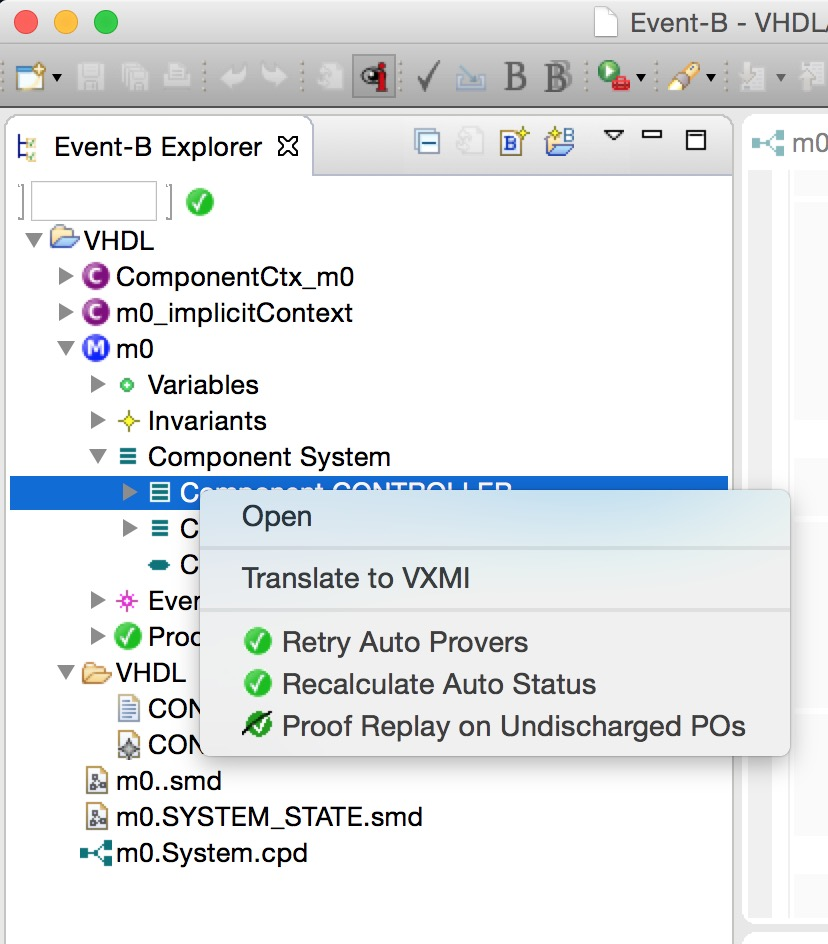
\includegraphics[width=512]{figures/vxmi-context_menu}
  \else
  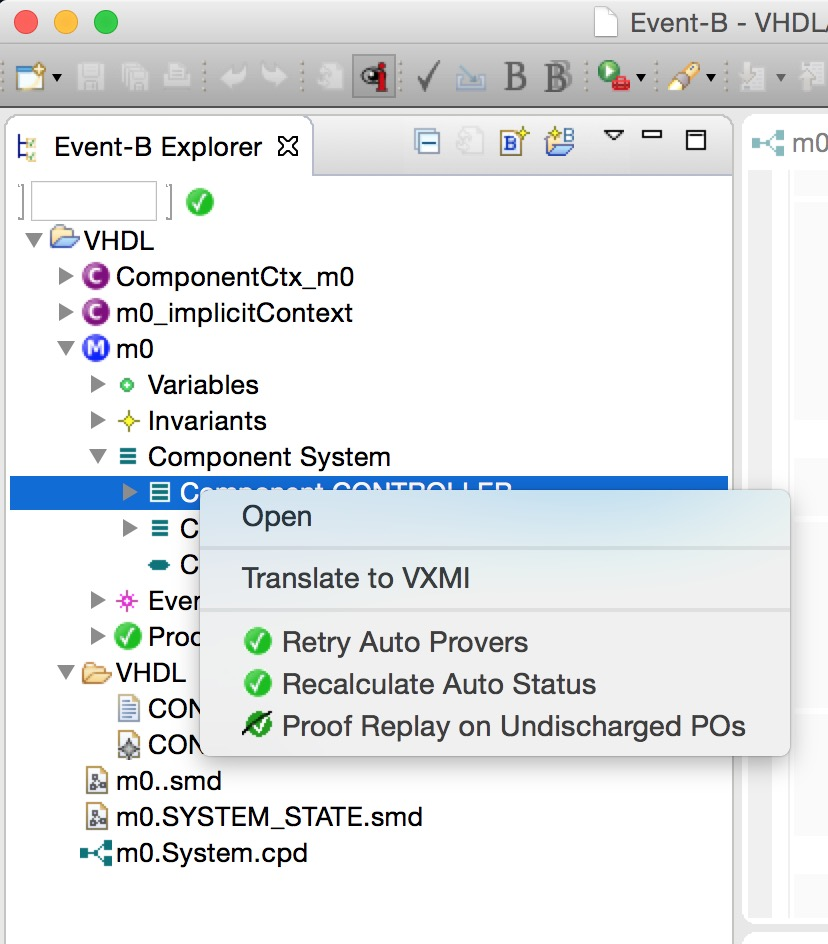
\includegraphics[width=0.5\textwidth]{figures/vxmi-context_menu}
  \fi
  \caption{VXMI generating from context menu}
  \label{fig:vxmi-context_menu}
\end{figure}
A \code{.vxmi} file with the same name of the source component is generated within the \code{VHDL} folder of the project.  To view the file in the \code{Event-B Explorer}, the users need to customise the view to \emph{disable} the filter on \code{All files and folders}.

\subsubsection{Generating VHDL from VXMI Tutorial}
\label{sec:vxmi-2-vhdl-tutorial}
The behavioural VHDL code can be generated from the context menu of a VXMI model as follows: \command{Right-click (on the VXMI model) -> Translate to VHDL}
\begin{figure}[!htbp]
  \centering
  \ifplastex
  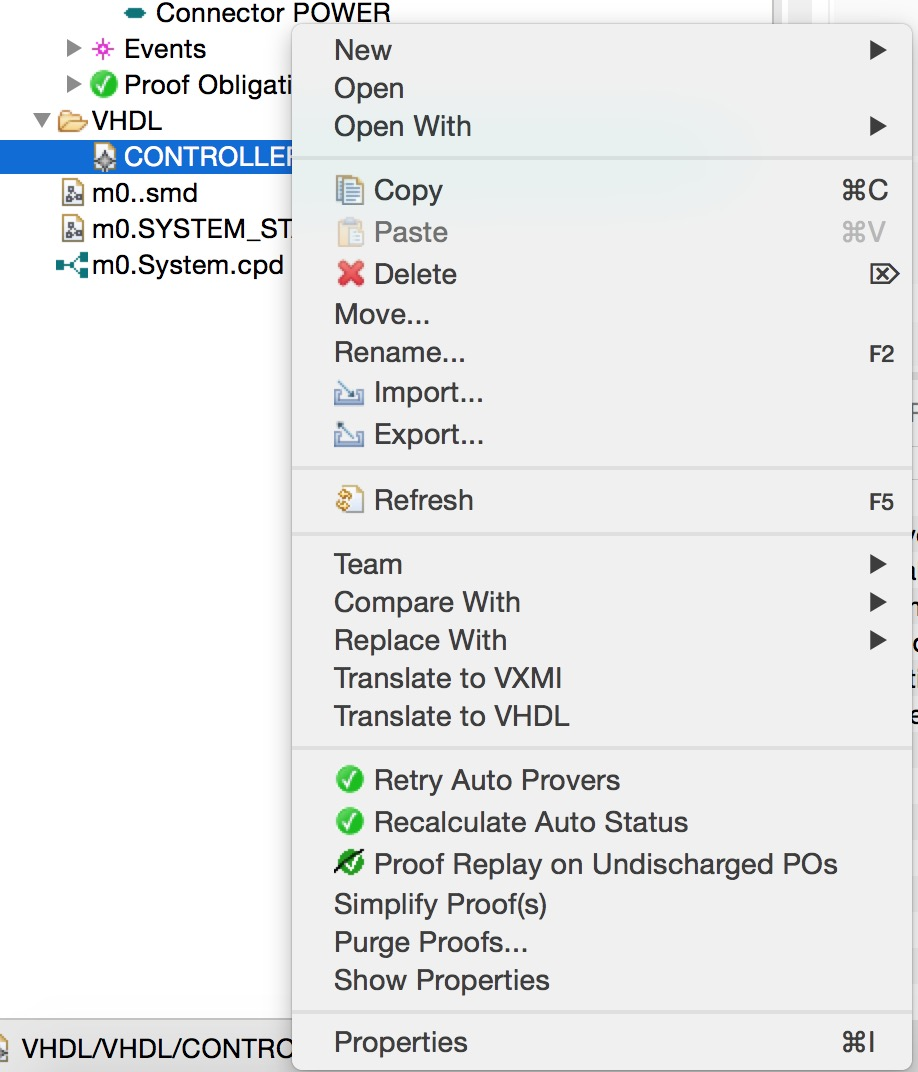
\includegraphics[width=512]{figures/vhdl-context_menu}
  \else
  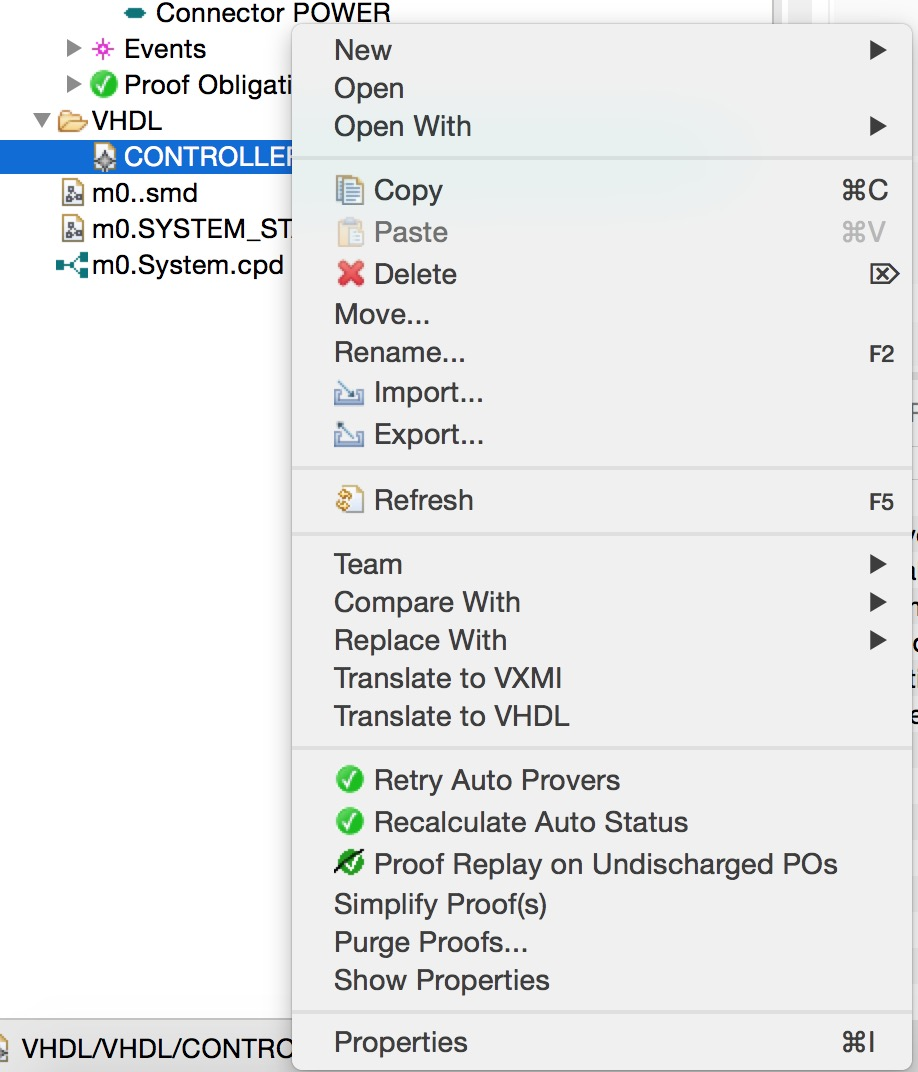
\includegraphics[width=0.5\textwidth]{figures/vhdl-context_menu}
  \fi
  \caption{VHDL generating from context menu}
  \label{fig:vhdl-context_menu}
\end{figure}
A \code{.vhdl} file with the same name of the source component is generated within the \code{VHDL} folder of the project.  To view the file in the \code{Event-B Explorer}, the users need to customise the view to \emph{disable} the filter on \code{All files and folders}.

%%% Local Variables:
%%% mode: latex
%%% TeX-master: "vhdl-user_manual"
%%% End:
